\label{sec:exp2}
De manera similar a la sección~\ref{sec:exp1}, en este experimento se nos planteo determinar los valores de los componentes planteados en nuestro modelo para una serie de distintos capacitores. Se redujo la resistencia $R_g$ del circuito anterior debido a que el componente resistivo es menor, dejando la resistencia en $R_g=1~k\Omega$. Se modifico la señal de entrada a una señal cuadrada para facilitar las medición. Ya que, como se explico en la sección~\ref{sec:Cap}, la señal en tensión resultante de este planteamiento sera una señal triangular (debido al efecto integrador de corriente del capacitor) sumada a la misma señal cuadrada (debido al efecto de la resistencia interna del capacitor), se podrá discernir y estimar los distintos componentes a través de la medición la señal a bornes del capacitor.

\begin{figure}[H]
    \centering
    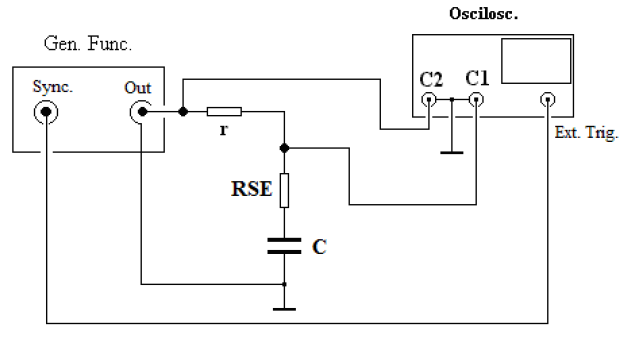
\includegraphics[width=0.7\linewidth]{Imagenes/exp2.png}
    \caption{Circuito experimento 2}
    \label{fig:exp2}
\end{figure}

Según lo anteriormente explicado podemos plantear los siguiente:
\begin{figure}[H]
    \centering
    \begin{minipage}{0.59\textwidth}
        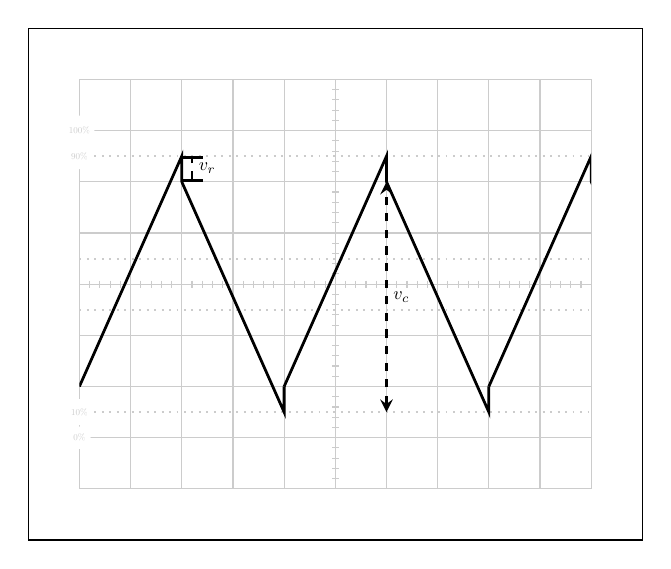
\begin{tikzpicture}[scale=0.65,every node/.style={transform shape}]
\def\res{0.5};%EscalaTemporal señal 1
\def\ind{1};%EscalaTemporal señal 2
\def\scalVa{1};%EscalaVertical señal 1
\def\frec{5};%EscalaVertical señal 2
\def\offseta{0};%Nivel de offset de la señal señal 1
\def\offsetb{};%Nivel de offset de la señal señal 2

%Lineas intermedias grilla
\foreach \x in {-5,-4.8,...,4.8,5}{
    \draw[gray!40,thin,shift={(\x,0)}] (0pt,2pt) -- (0pt,-2pt);
}
\foreach \y in {-4,-3.8,...,3.8,4}{
    \draw[gray!40,thin,shift={(0,\y)}] (2pt,0pt) -- (-2pt,0pt);
}
\foreach \a [evaluate={\y=\a*0.5}] in {-5,-1,1,5}{
    \draw[gray!40,line width=0.7pt,dotted] (-5,\y) -- (5,\y);
}

%Grilla
\draw[thin,gray!40] (-5,-4) grid (5,4);
\node[fill=white,text=gray!40,circle,scale=0.5] at (-5,3) {$100\%$};
\node[fill=white,text=gray!40,circle,scale=0.5] at (-5,2.5) {$90\%$};
\node[fill=white,text=gray!40,circle,scale=0.5] at (-5,-2.5) {$10\%$};
\node[fill=white,text=gray!40,circle,scale=0.5] at (-5,-3) {$0\%$};
\draw[black] (-6,-5) rectangle(6,5);

%Señal 1
\clip (-5,-4) rectangle (5,4);
\foreach [evaluate={\a=\c+2}] \c in{-5,-1,3}{
    \draw[line width=1pt](\c,-2)--(\a,2.5)--(\a,2){};
    \draw[line width=1pt](\a,2)--(\a+2,-2.5)--(\a+2,-2){};
}
\draw[line width=1pt,dashed,stealth-stealth](1,-2.5)--(1,2) node[midway,right]{$v_c$};
\draw[line width=1pt,dashed,stealth-stealth,|-|](-2.8,2)--(-2.8,2.5)node[anchor=north west]{$v_r$};
\end{tikzpicture}
        \label{fig:enter-label}
    \end{minipage}
    \begin{minipage}{0.29\textwidth}
       \begin{circuitikz}[scale=1,every node/.style={transform shape},style=american]
\draw (0,2)to[open,v=$v_i$,o-o](0,-2)--(3,-2)to[capacitor=$C$](3,0)to[R=$r_c$](3,2) (0,2)to[R=$R_g$,i=$i_{(t)}$](3,2);
\draw[line width=0.7pt,dashed] (2.3,-1.8)rectangle(3.3,1.8);
\draw (3.7,0)to[open,v=$v_c$](3.7,-2)  (3.7,2)to[open,v=$v_r$](3.7,0);
\end{circuitikz}

\end{minipage}
\caption{Análisis del circuito equivalente de un capacitor}
\end{figure}
Tomando los valores de los tramos de la señal correspondiente a los distintos componentes, se pude calcular el valor de la resistencia de la siguiente manera:
\begin{equation}
    r_c=\frac{v_r}{i}
\end{equation}

\unsubsubsection{Mediciones}
La señal cuadrada utilizada fue establecida en los siguientes valores: 
\begin{itemize}
    \item $V_{pp}=20~V$
    \item  $F_{rec}=10 ~KHz$
\end{itemize}

Se procedió a medir sobre los puntos establecidos, obteniendo los siguientes datos:
\begin{figure}[H]
    \centering
    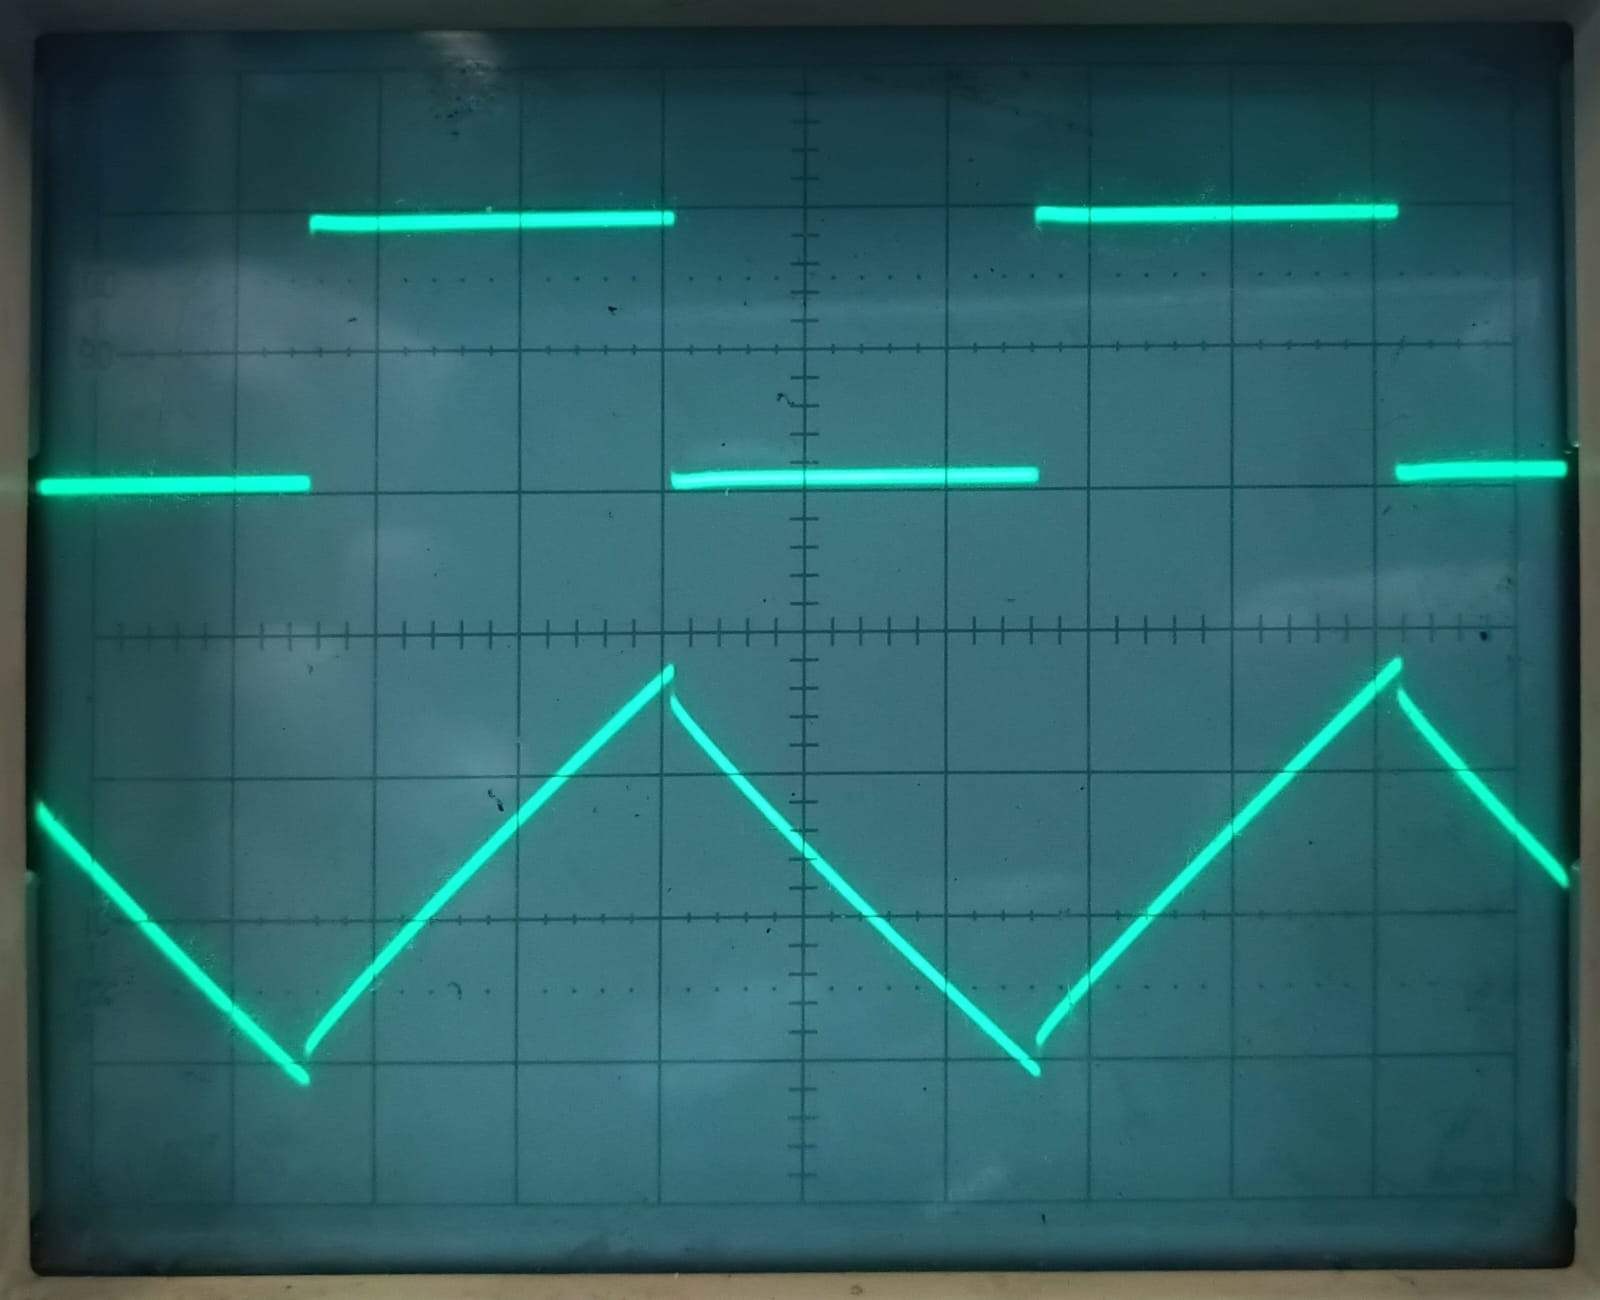
\includegraphics[width=0.6\textwidth]{Imagenes/MedExp2.jpeg}
    \caption{Mediciones de la señal de salida vs entrada del experimento 2}

\end{figure}
\begin{table}[H]
    \centering
    \begin{tabular}{|c|c|c|c|}
    \hline
        $f$ & \multicolumn{3}{c|}{$10~kHz$}\\
    \hline
        $C_{nom}$ & $1~\mu F$ & $2.2~\mu F$ & $4.7~\mu F$ \\ 
    \hline
        $r$ & \multicolumn{3}{c|}{$1~k\Omega$}\\
    \hline
        $e_{pp}~(Canal~2)[V]$ & 20 & 20 & 20\\
    %\hline
        $I=\cfrac{e_{pp}}{r} ~[mA]$ & 18.5 & 18.5 & 18.5 \\
    %\hline    
        $e_R~[mV]$ & 36 & 149.85 & 50 \\
    %\hline    
        $RSE = \cfrac{e_R}{I} ~[\Omega]$ & 1.94 & 7.3 & 2.7 \\
    \hline    
    
        \end{tabular}
        \def\tablename{Tabla} 
        \caption{Tabla de parámetros para distintos capacitores}
        \label{tab:exp2}
\end{table}

\unsubsubsection{Comprobación}
Utilizando un medidor RLC se comprobaron los valores nominales de los 3 capacitores utilizados:

\begin{figure}[H]
\centering
    \begin{minipage}{0.29\textwidth}
    \centering
    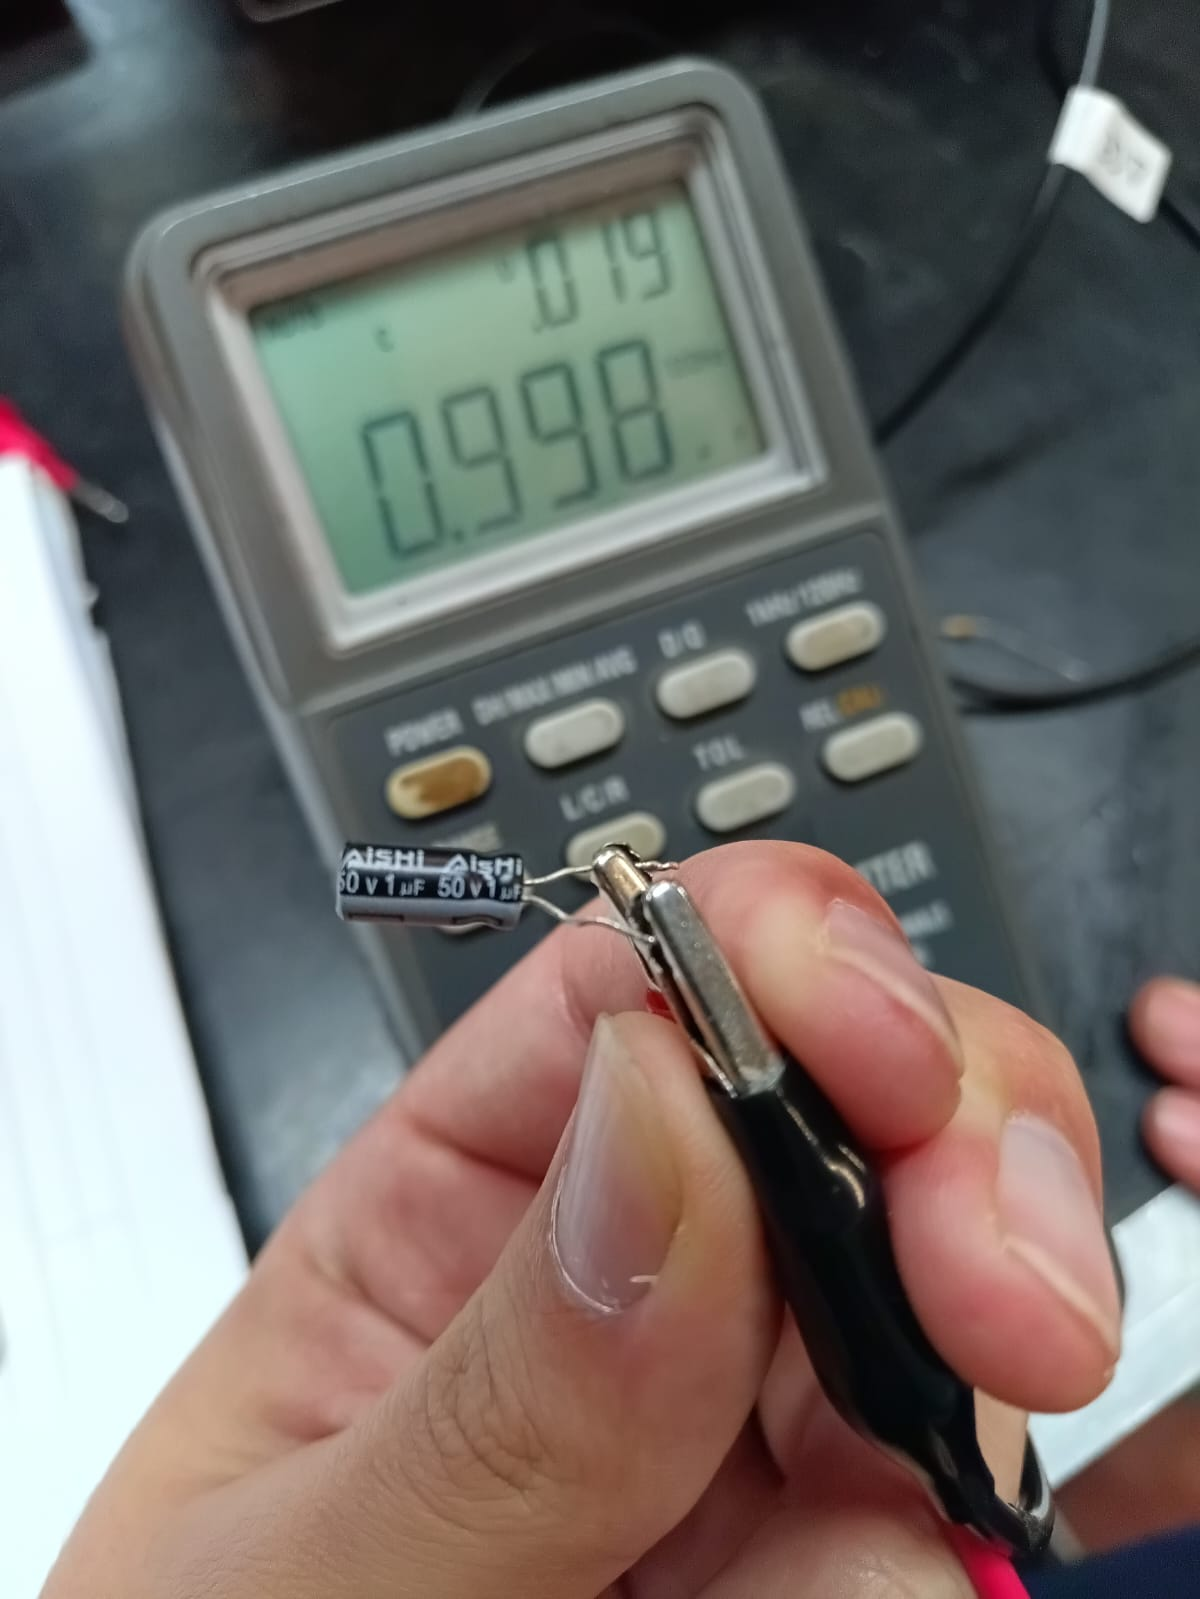
\includegraphics[width=\textwidth,trim={0cm 10cm 0cm 0cm},clip]{Imagenes/MedCap3Exp2.jpeg}
    \caption*{$C=1~\mu F$}
    \end{minipage}
    \hspace*{\fill}
    \begin{minipage}{0.29\textwidth}
    \centering
    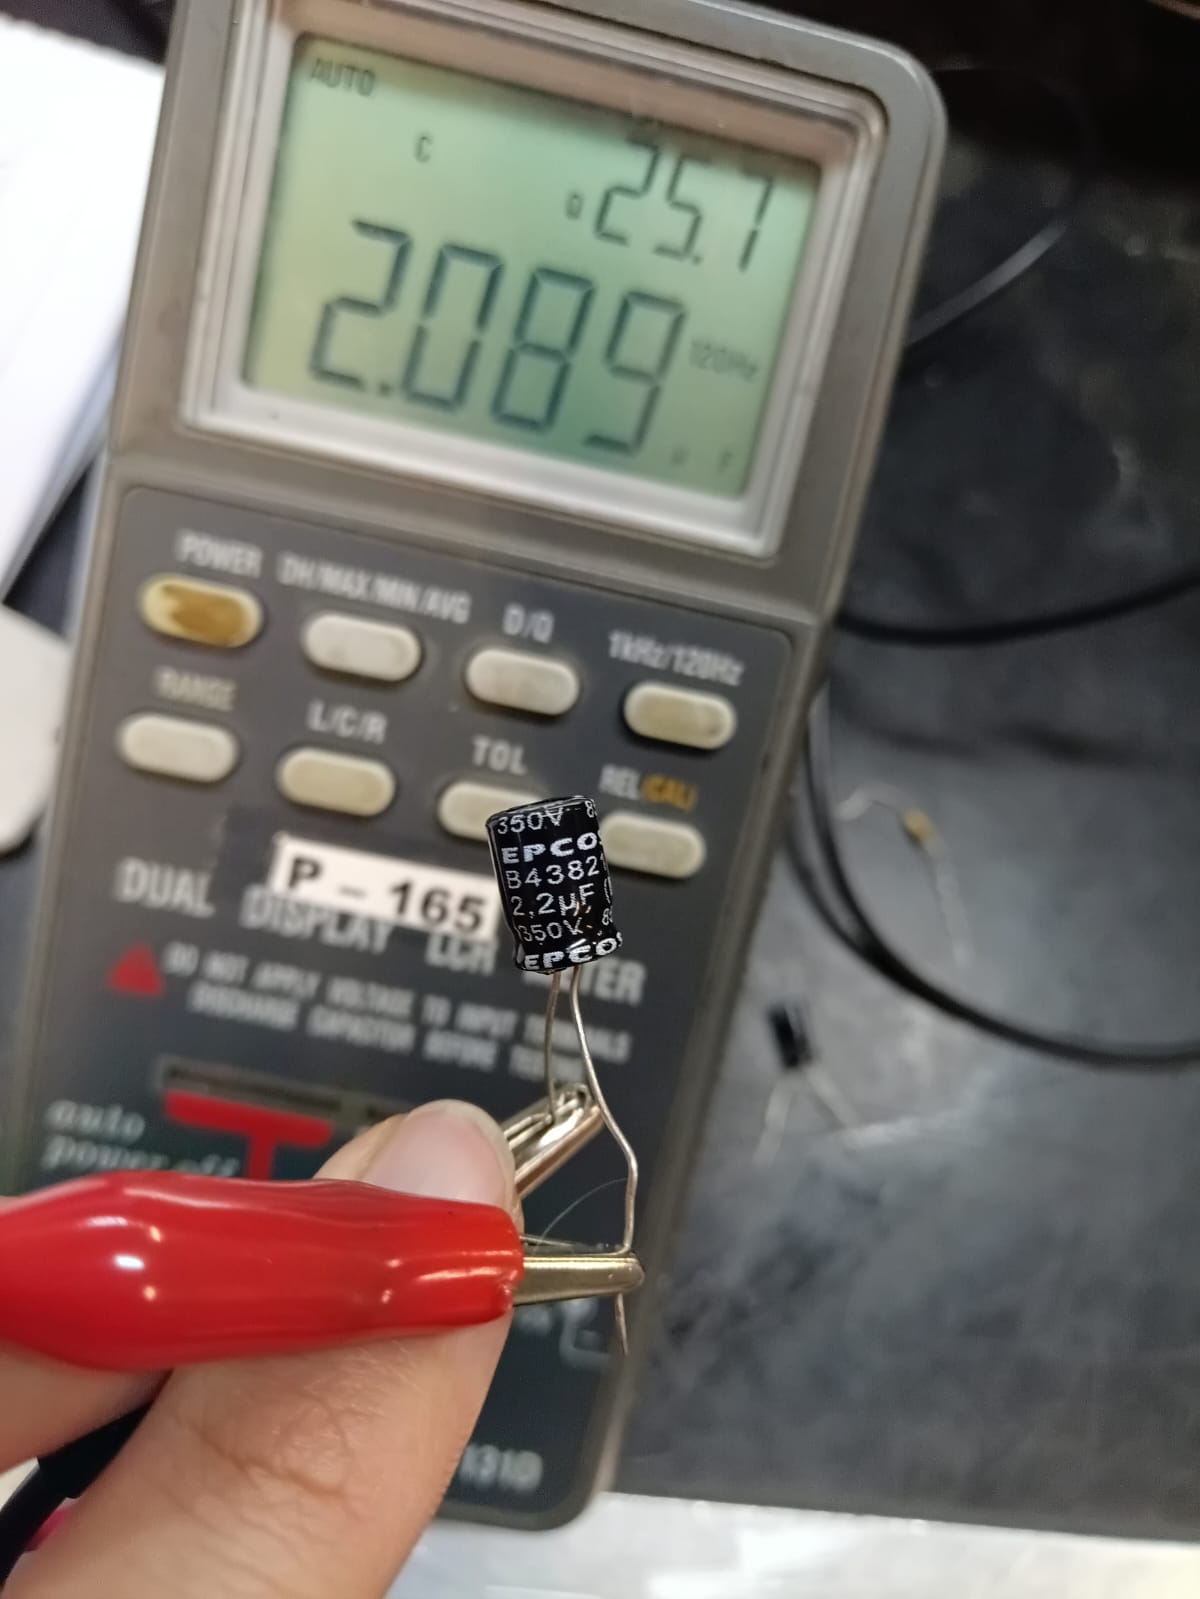
\includegraphics[width=\textwidth,trim={0cm 10cm 0cm 0cm},clip]{Imagenes/MedCap1Exp2.jpeg}
    \caption*{$C=2.2~\mu F$}
    \end{minipage}
    \hspace*{\fill}
    \begin{minipage}{0.29\textwidth}
    \centering
    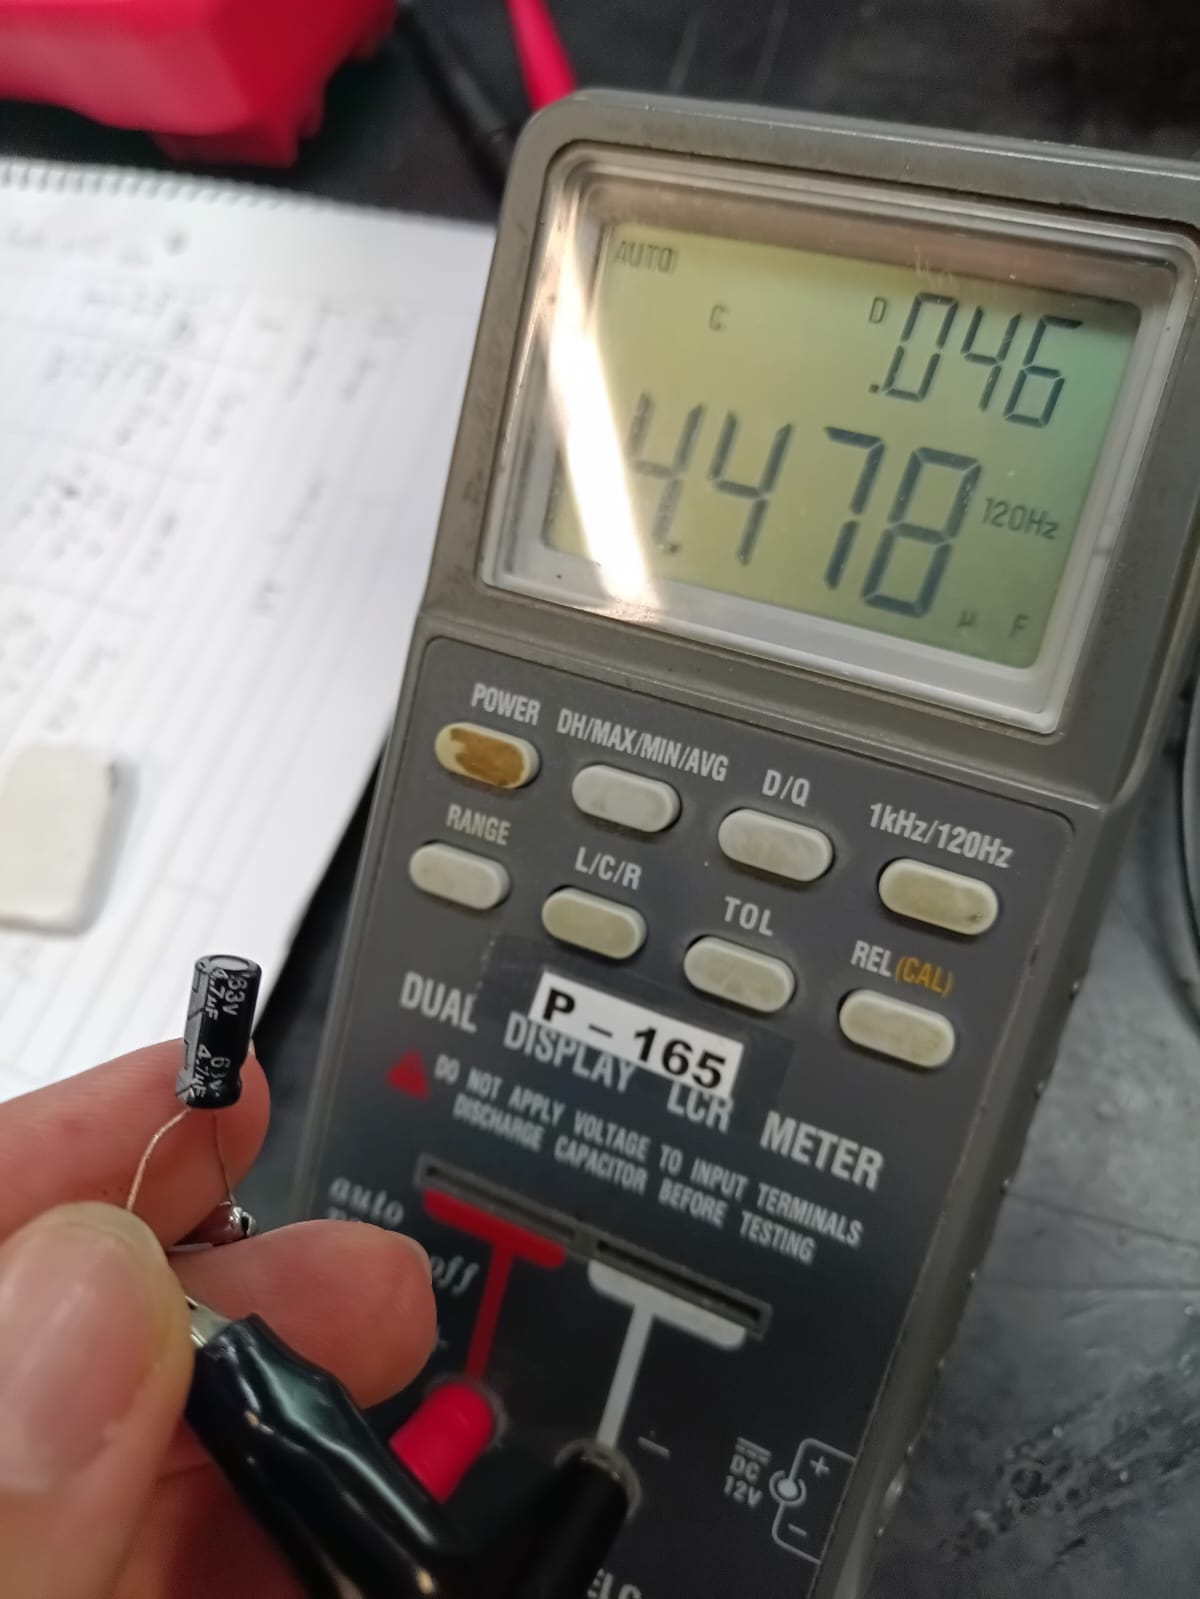
\includegraphics[width=\textwidth,trim={0cm 10cm 0cm 0cm},clip]{Imagenes/MedCap2Exp2.jpeg}
    \caption*{$C=4.7~\mu F$}
    \end{minipage}
    \caption{Mediciones de los capacitores del experimento 2}
\end{figure}